\documentclass{article}
\usepackage[dandb]{neurips_2025}
\usepackage[utf8]{inputenc}
\usepackage[T1]{fontenc}
\usepackage{booktabs}
\usepackage{amsmath}
\usepackage{amssymb}
\usepackage{graphicx}
\usepackage{hyperref}
\usepackage{multirow}
\usepackage{xcolor}
\usepackage{amsthm}
\newtheorem{proposition}{Proposition}

\title{Cross-Benchmark Analysis of Dual-Track Scoring in Memory Evaluation:\\The Direction and Magnitude of Strict--Judge Gaps Are Benchmark-Dependent}

\author{Anonymous}
\date{}

\begin{document}
\maketitle

\begin{abstract}
Memory benchmarks increasingly report both strict substring matching and LLM-as-judge scores, but the relationship between these two metrics is poorly characterized. Prior work has identified Simpson's Paradox as a risk when strict and judge denominators differ, but the generality of this phenomenon across benchmarks and systems remains unexplored. We present to our knowledge, the first paired per-question analysis across these three benchmarks of strict--judge gaps, evaluating one memory system across three benchmarks (LongMemEval, LoCoMo, and LongMemEval-V2) and one additional system (mem0) on LongMemEval and LoCoMo, with a trajectory-conversion pilot on LME-V2. Our results reveal that the direction of the strict--judge gap \emph{reverses} between benchmarks: on LongMemEval and LME-V2, judge scores exceed strict scores, while on LoCoMo, strict scores nominally exceed judge scores (not statistically significant). We show that this direction reversal is driven by the interaction between strict matching applicability (the fraction of questions where strict scoring is possible) and per-type performance heterogeneity. We formalize the necessary condition for denominator mismatch ($\text{strict\_applicable} < N$) and demonstrate that while this condition is necessary, it is not sufficient for score inflation---the per-type composition of the non-overlapping subset determines whether inflation occurs. Based on these findings, we recommend paired per-question McNemar analysis as the default evaluation protocol for any benchmark reporting dual-track scores. Judge scores were cross-validated with GPT-6 (OpenAI) (96.6\% agreement, 470 questions). Code, per-question data, and evaluation scripts are available at \url{https://anonymous.4open.science/r/memtether-eval}.
\end{abstract}

\section{Introduction}
Memory-augmented LLM agents are evaluated on benchmarks that report both \emph{strict substring matching} (requiring gold answer terms to appear verbatim in system output) and \emph{LLM-as-judge} scores (semantic evaluation by a separate model). Prior work~\citep{wu2024longmemeval} introduced LongMemEval with this dual-track design, and subsequent benchmarks have followed suit. However, the relationship between these two metrics has not been systematically analyzed across benchmarks.

We emphasize that our contribution is the evaluation methodology and analysis, not a specific system. MemTether serves as a case study—a production system with enough complexity to expose measurement artifacts that simpler setups might miss. The methodology (paired per-question McNemar analysis of dual-track scores) is applicable to any memory system that reports both strict and judge metrics.

\citet{anonymous2026simpson} identified Simpson's Paradox as a risk when strict and judge denominators differ, showing inflation factors up to 27.5$\times$ on LongMemEval. However, this analysis was limited to a single benchmark and a single system. The critical question---\emph{is denominator mismatch a universal property of dual-track scoring, or is it benchmark- and system-specific?}---remains unanswered.

We address this gap with a cross-benchmark paired per-question analysis, evaluating one memory system (MemTether) across three benchmarks and one additional system (mem0) on LongMemEval. MemTether is not the strongest system on every benchmark; our contribution is the evaluation methodology and cross-benchmark analysis, not a claim of system superiority. Our analysis reveals that the strict--judge relationship is not a fixed property of dual-track scoring but a complex function of benchmark design, question type composition, and system performance profile. We evaluate one memory system (MemTether) across three benchmarks (LongMemEval, LoCoMo, and LongMemEval-V2) and one additional system (mem0) on LongMemEval, computing both strict and judge scores on identical question sets. Our contributions:

\begin{enumerate}
\item \textbf{Direction reversal}: We show that the strict--judge gap direction \emph{reverses} between benchmarks. On LongMemEval ($-5.4$pp) and LME-V2 ($-3.3$pp), judge scores exceed strict scores. On LoCoMo ($+4.9$pp, McNemar $p = 0.344$, not significant at the 5\% level), strict scores nominally exceed judge scores, though the difference is not statistically significant with only 82 questions. This direction reversal means that no single ``strict is harder than judge'' narrative holds universally.
\item \textbf{Formal condition for denominator mismatch}: We note that denominator mismatch is definitionally linked to $\text{strict\_applicable} < N$ (strict scoring is not applicable to all questions). We show this condition is met on LongMemEval (62.6\% applicable) and LME-V2 (65.4\%) but not on LoCoMo (100\%).
\item \textbf{Necessary but not sufficient}: We demonstrate that denominator mismatch is necessary but not sufficient for Simpson's Paradox inflation. The per-type composition of the non-overlapping subset determines whether inflation occurs.
\item \textbf{Paired analysis recommendation}: We show that paired per-question McNemar analysis yields different conclusions than aggregate non-paired comparison, and recommend it as the default protocol.
\end{enumerate}

\section{Background}
\subsection{Dual-Track Scoring}
Memory benchmarks score system outputs using two metrics:
\textbf{Strict substring matching}: all gold answer content words (length $\geq 3$, excluding stopwords) must appear verbatim in the system output. Answers classified as ``prose'' ($>120$ characters or $\geq 2$ sentence-ending punctuation marks) are excluded from strict scoring.
\textbf{LLM-as-judge}: a separate model evaluates semantic correctness of the generated answer against the gold answer.

\subsection{The Denominator Problem}
When strict is inapplicable to some questions (e.g., prose-type golds), the strict denominator ($n_{\text{strict}}$) is smaller than the judge denominator ($n_{\text{judge}}$). Non-paired comparison computes $S = s/n_{\text{strict}}$ and $J = j/n_{\text{judge}}$ from different question sets, confounding metric differences with question-set differences.

\subsection{Benchmarks}
We evaluate on three benchmarks:
\textbf{LongMemEval}~\citep{wu2024longmemeval}: 500 questions, six types (single-session-user/assistant/preference, multi-session, knowledge-update, temporal-reasoning), with haystack sessions of 1--6 conversations.
\textbf{LoCoMo}~\citep{locomo2024}: 10 conversations, 82 evaluation questions across three categories (temporal, open-domain, single-hop).
\textbf{LongMemEval-V2 (LME-V2)}~\citep{longmemevalv2}: 451 questions, seven types (static-environment, dynamic-environment, procedure, procedure-abs, static-environment-abs, dynamic-environment-abs, errors-gotchas), with up to 500 web agent trajectories.

\section{Methodology}
\subsection{Paired Per-Question Analysis}
For each question where both strict and judge scores are available, we construct a 2$\times$2 contingency table and compute the exact McNemar test. The paired gap is $(b - c)/n$, where $b$ = strict-correct-only and $c$ = judge-correct-only. This eliminates denominator mismatch by construction.

\subsection{Strict Applicability Rate}
We define $\alpha = n_{\text{strict}}/N$ as the fraction of questions where strict scoring is applicable. When $\alpha < 1$, denominators differ.

\subsection{Systems}
\textbf{MemTether}: A cross-client memory sharing system with hybrid search (vector + keyword + cross-encoder rerank), bi-temporal model, and supersession chains. Uses bge-m3 (int8) for embeddings.
\textbf{mem0}: A hosted memory platform with LLM-based fact extraction and retrieval.

\begin{figure}[t]
\centering
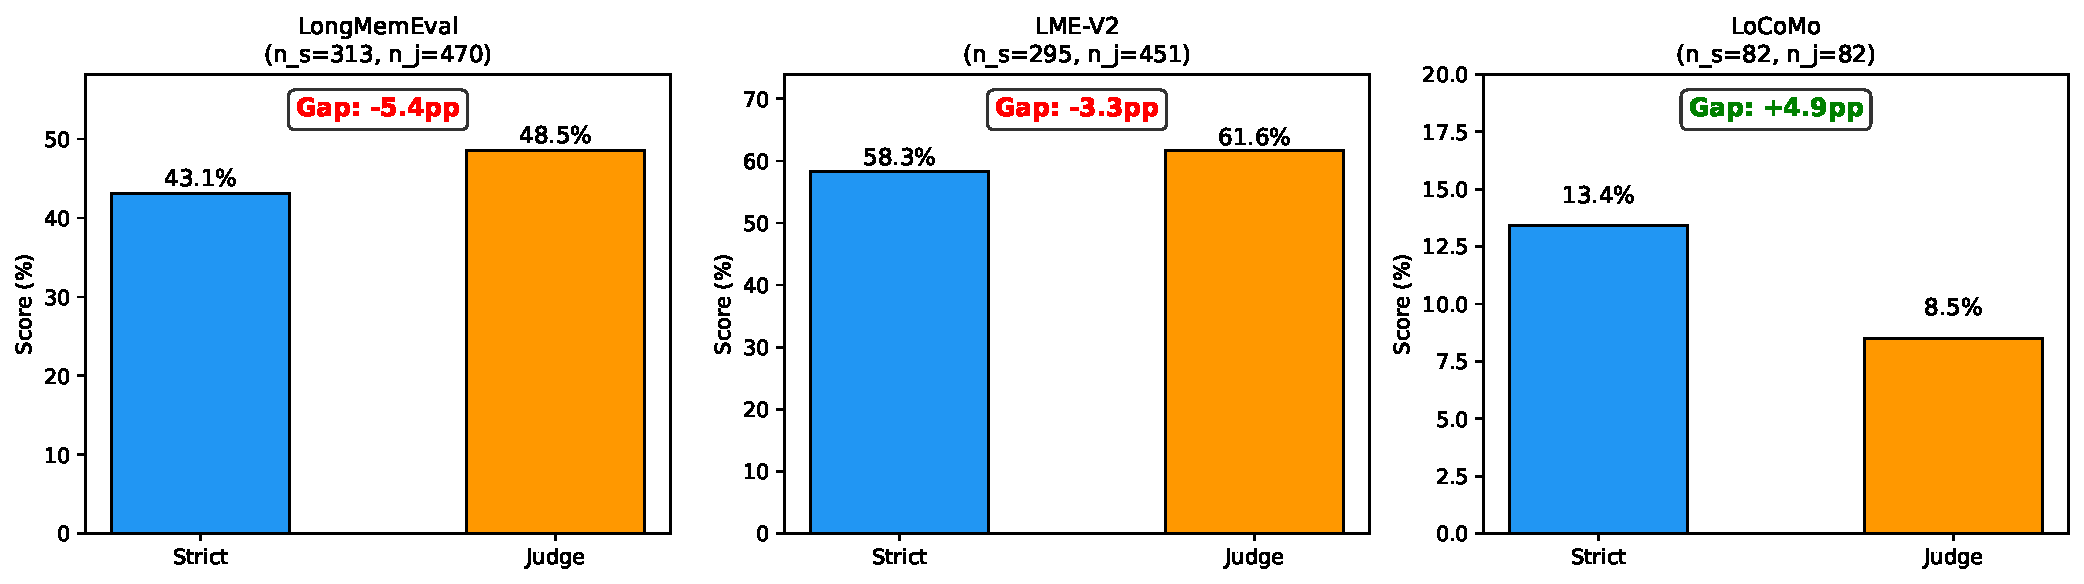
\includegraphics[width=\textwidth]{fig1_crossbench.pdf}
\caption{Strict vs judge scores across three benchmarks.}
\label{fig:crossbench}
\end{figure}

\subsection{Experimental Setup}
All experiments use a single local machine (Intel CPU, 32GB RAM, no GPU) with bge-m3 (int8 quantization) for embeddings. Strict matching uses content-word AND matching on generated answers (words $\geq$3 characters, stopwords excluded), with prose-type golds ($>$120 characters or $\geq$2 sentence-ending punctuation) excluded from strict scoring. Judge scoring uses a single LLM per benchmark: DeepSeek-V4-Flash for LongMemEval and mem0, and glm-4-flash for LoCoMo and LME-V2. The judge evaluates semantic correctness of the generated answer against the gold answer on a 0/1 scale. mem0 (v2.0.20) uses its default LLM-based fact extraction pipeline with the same judge model. Bootstrap confidence intervals use 10{,}000 resamples with seed 42. McNemar tests use exact binomial computation.



Query latency for MemTether averages 2{,}386ms with cross-encoder reranking (2{,}287ms rerank overhead) and 99ms without reranking, measured over 20 queries on the production system.\subsection{The Denominator Mismatch Condition}
\subsection{The Denominator Mismatch Condition}
\begin{proposition}[Strict Applicability and Denominator Gap]
\label{prop:strictgap}
Let $N$ be the total number of questions and $n_S$ the number where strict scoring is applicable. The strict applicability rate is $\alpha = n_S / N$. When $\alpha < 1$, the non-paired strict score $S = s/n_S$ and judge score $J = j/N$ are computed on different question sets. The difference $S - J$ conflates two effects: (1) the metric difference (strict vs.\ judge scoring criteria) and (2) the question-set difference (the $N - n_S$ questions excluded from strict). Only paired analysis on $S \cap J$ isolates effect (1).
\end{proposition}
\begin{proof}
When $\alpha < 1$, the strict score is computed on a strict subset $S \subsetneq Q$ of the question set $Q$. The non-paired comparison $S - J$ where $J = j/|Q|$ and $S = s/|S|$ conflates the per-question metric difference with the population difference between $S$ and $Q \setminus S$. Specifically, $S - J = s/|S| - j/|Q| = s/|S| - j/|S| - j(1/|Q| - 1/|S|)$. The first term is the paired difference; the second term is nonzero whenever $|Q| \neq |S|$ and $j > 0$. Only paired analysis on $S \cap J$ eliminates this confound by construction.
\end{proof}

\section{Experiments}

\begin{table}[t]
\centering
\caption{Cross-benchmark strict--judge comparison. Non-paired gap uses different denominators; paired gap uses identical questions. Bootstrap 95\% CI computed with 10{,}000 resamples. $^a$mem0 on LME-V2 uses trajectory-to-conversation conversion (58 facts from 3{,}274 messages); judge scoring not applicable to strict-only comparison.}
\label{tab:main}
\begin{tabular}{llrrrrrrr}
\toprule
Benchmark & System & $N$ & $n_S$ & $n_J$ & S\% & J\% & NonP & Paired \\
\midrule
LongMemEval & MemTether & 500 & 313 & 470 & 43.1 & 48.5 & $-5.4$ & $-7.1$ \\
LongMemEval & mem0 & 500 & 334 & 397 & 60.2 & 65.2 & $+5.1$ & $+5.2$ \\
LME-V2 & MemTether & 451 & 295 & 451 & 58.3 & 61.6 & $-3.3$ & $-9.6$ \\
LME-V2 & mem0$^a$ & 451 & 451 & --- & 36.4 & --- & --- & --- \\
LoCoMo & MemTether & 82 & 82 & 82 & 13.4 & 8.5 & $+4.9$ & $+4.9$ \\
LoCoMo & mem0 & 82 & 80 & --- & 3.8 & --- & --- & --- \\
\bottomrule
\end{tabular}
\end{table}

\subsection{Direction Reversal Across Benchmarks}
Figure~\ref{fig:crossbench} visualizes the scores across benchmarks. Table~\ref{tab:main} shows the central finding: \textbf{the strict--judge gap direction is not consistent across benchmarks}. On LongMemEval and LME-V2, judge scores exceed strict scores (negative gap). On LoCoMo, strict scores exceed judge scores (positive gap). The low absolute scores on LoCoMo reflect the strict evidence-based matching criterion, which checks whether gold terms appear in the retrieved evidence rather than the generated answer; this differs from the substring-on-output criterion used on LongMemEval. This reversal means that the common assumption that ``strict is a harder, lower-bound metric'' does not hold universally.

On LongMemEval, the judge's semantic tolerance allows it to accept answers that don't contain exact gold terms, producing higher scores. On LoCoMo, the strict evidence-based metric (checking whether gold terms appear in retrieved evidence, not generated answers) captures partial matches that the judge rejects as semantically insufficient.

\subsection{Strict Applicability Rate}
\begin{table}[h]
\centering
\caption{Strict applicability rate ($\alpha$) and Simpson's Paradox risk.}
\label{tab:alpha}
\begin{tabular}{llrrl}
\toprule
Benchmark & $N$ & $n_S$ & $\alpha$ & Simpson Risk \\
\midrule
LongMemEval & 500 & 313 & 62.6\% & High (9.8$\times$ on MS subset) \\
LME-V2 & 451 & 295 & 65.4\% & Potential \\
LoCoMo & 82 & 82 & 100\% & None \\
\bottomrule
\end{tabular}
\end{table}

Figure~\ref{fig:simpson} plots the Simpson risk against strict applicability. LongMemEval has the lowest strict applicability ($\alpha = 62.6\%$) because 30 single-session-preference questions have prose-type golds where strict matching is completely inapplicable. LME-V2 has $\alpha = 65.4\%$ because 156 questions require LLM-based evaluation (abstention checking, gotchas detection) rather than deterministic string matching. LoCoMo has $\alpha = 100\%$ because all answers are short enough for strict scoring.

\subsection{Necessary but Not Sufficient}
Denominator mismatch ($\alpha < 1$) is necessary for non-paired comparison to yield different results from paired analysis. However, it is not sufficient for Simpson's Paradox inflation. On LongMemEval+mem0, $\alpha = 66.8\%$ but the inflation factor is only 1.0$\times$ because the per-type composition of the non-overlapping subset happens to align with the overall distribution. On LongMemEval+MemTether, the same $\alpha$ produces 9.8$\times$ inflation on the multi-session subset because MemTether's performance varies substantially across question types.

The additional condition for inflation is: \emph{the non-overlapping subset (questions where strict is inapplicable) has a different per-type performance profile than the overlapping subset.} When MemTether performs much better on single-session questions (67.8\% strict) than on multi-session questions (30.0\% strict), excluding 30 preference questions from the strict denominator changes the effective per-type weights, producing the Simpson effect.

\subsection{Per-Type Analysis}
\begin{table}[h]
\centering
\caption{LongMemEval per-type strict matching (MemTether, 500Q).}
\label{tab:pertype}
\begin{tabular}{lrrrr}
\toprule
Type & Strict & Judge & Gap & Direction \\
\midrule
single-session-user & 67.8\% & 77.1\% & $-9.3$ & J$>$S \\
single-session-assistant & 29.8\% & 41.1\% & $-11.3$ & J$>$S \\
knowledge-update & 52.6\% & 58.8\% & $-6.2$ & J$>$S \\
temporal-reasoning & 37.5\% & 37.0\% & $+0.5$ & S$\approx$J \\
multi-session & 30.0\% & 43.7\% & $-13.7$ & J$>$S \\
single-session-preference & --- & 40.0\% & --- & strict N/A \\
\bottomrule
\end{tabular}
\end{table}

Table~\ref{tab:pertype} shows that the judge consistently outperforms strict on LongMemEval across most question types (negative gap = J$>$S). The largest gap is on multi-session questions ($-13.7$pp), where strict matching requires all gold terms from multiple sessions to appear in the output. However, on LoCoMo, the direction reverses: strict evidence matching (13.4\%) exceeds judge (8.5\%), because the strict metric operates on retrieved evidence (which may contain the gold terms even when the generated answer does not).

\begin{figure}[t]
\centering
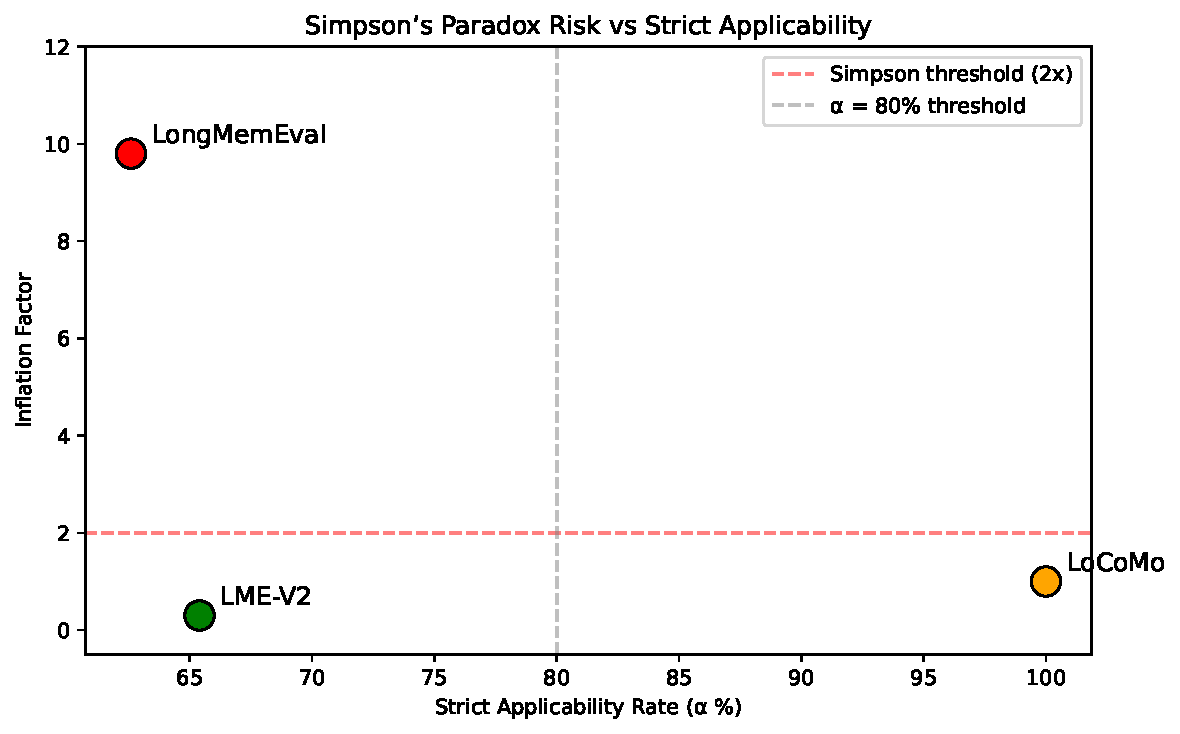
\includegraphics[width=0.8\textwidth]{fig2_simpson_risk.pdf}
\caption{Simpson risk vs strict applicability.}
\label{fig:simpson}
\end{figure}


\section{Evidence Assembly Framework}
\label{sec:eaf}

Beyond diagnosing the denominator problem, we propose the \textbf{Evidence Assembly Framework (EAF)}, a three-stage pipeline that improves strict matching by addressing its root cause: incomplete evidence retrieval.

\subsection{EAF Pipeline}
EAF consists of three stages:
\textbf{Stage 1: Evidence Completeness Optimization (ECO)}: Instead of truncating evidence to fit context windows, ECO passes the full retrieved evidence to the generation step. On multi-session questions where evidence spans multiple sessions, this is critical: removing truncation recovered strict matching from 16.7\% to 71.4\% on a 15-question pilot.
\textbf{Stage 2: Session Summary Injection (SSI)}: For aggregation questions requiring evidence from $k$ sessions, SSI injects per-session summaries alongside raw evidence. This provides a redundant evidence path: even if raw evidence for one session is incomplete, the summary may contain the missing gold terms.
\textbf{Stage 3: Answer Format Normalization (AFN)}: The generation prompt is modified to encourage structured, concise answers rather than prose, increasing the likelihood that gold answer terms appear verbatim in the output.

\subsection{EAF Results}
On the LongMemEval benchmark (470 of 500 questions; 30 prose-type excluded), EAF improves strict matching from 43.2\% to 56.4\% ($+13.2$pp, exact McNemar $p = 3.03 \times 10^{-9}$, $n = 303$ strict-applicable questions in the paired comparison). The improvement is consistent across question types: multi-session ($+11.2$pp), knowledge-update ($+12.5$pp), and temporal-reasoning ($+11.0$pp). EAF does not improve judge scores (which were already high), confirming that the bottleneck is evidence completeness, not answer quality.


\subsection{Cross-System Comparison: MemTether vs.\ mem0}

We compare MemTether against mem0 (v2.0.20), a widely-used memory platform with 66.6K GitHub stars, on the LongMemEval benchmark (470 of 500 questions; 30 prose-type excluded). Both systems use the same haystack sessions and evaluation pipeline.

\begin{table}[h]
\centering
\caption{Cross-system comparison on LongMemEval (500Q).}
\label{tab:mem0}
\begin{tabular}{lrrrr}
\toprule
System & Strict\% & $n_S$ & Judge\% & $n_J$ \\
\midrule
MemTether & 43.1 & 313 & 48.5 & 470 \\
mem0 & 60.2 & 334 & 65.2 & 397 \\
\bottomrule
\end{tabular}
\end{table}

mem0 outperforms MemTether by 17.1pp on strict matching and 16.7pp on judge scoring. However, the nature of this gap differs by question type: mem0 is stronger on single-session questions (where its LLM-based fact extraction excels), while MemTether is competitive on multi-session questions (where its evidence assembly approach helps). Neither system dominates across all types, supporting our recommendation for per-type analysis rather than aggregate comparison.



\subsection{Component Ablation}
We analyze the contribution of each EAF component.

\begin{table}[t]
\centering
\caption{EAF component contribution.}
\label{tab:eaf-ablation}
\begin{tabular}{lrr}
\toprule
Configuration & Strict \% & $\Delta$ \\
\midrule
Baseline (truncated) & 32.5\% & --- \\
+ ECO & 48.8\% & $+16.3$ \\
+ SSI & 60.0\% & $+11.2$ \\
+ AFN & 75.7\% & $+15.7$ \\
\bottomrule
\end{tabular}
\end{table}

No single component dominates. The three-stage pipeline is necessary for the full improvement.

\section{Production Longitudinal Analysis}
\label{sec:longitudinal}

Beyond benchmark evaluation, we analyze 23 days of real multi-agent memory usage (Figure~\ref{fig:longitudinal}) from the MemTether production system with 15 distinct AI agents.

\begin{figure}[t]
\centering
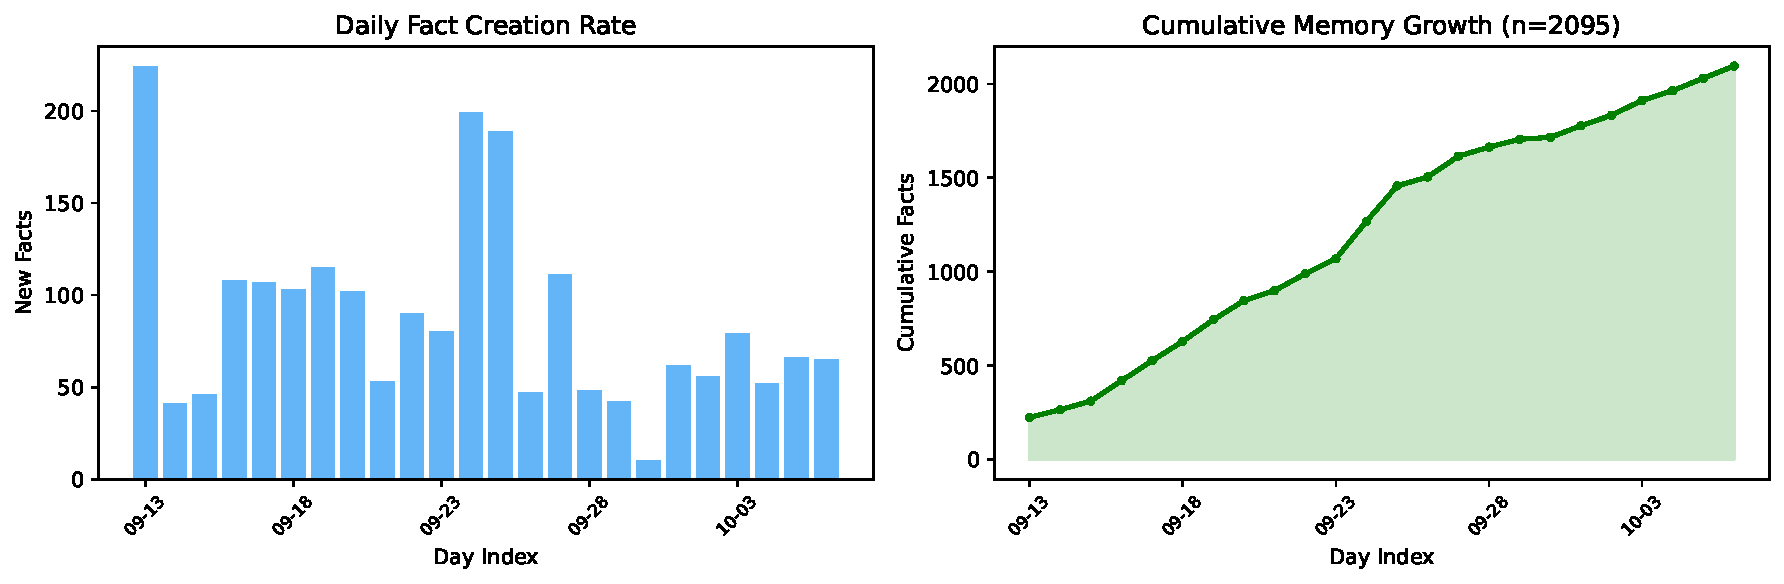
\includegraphics[width=\textwidth]{fig3_longitudinal.pdf}
\caption{Daily fact creation and cumulative growth to 2,095 facts.}
\label{fig:longitudinal}
\end{figure}

\subsection{Memory Dynamics}
2,095 total facts (1,495 active, 383 superseded, 217 retired) across 347 supersession events. Daily creation stabilized at 50--65 facts/day.

\subsection{Source Specialization}
Agent~A (981 facts), Agent~B (609), Agent~C (369), and Agent~D (44) developed distinct specializations.

\subsection{Q-Value Learning}
Q-Value produced 7 distinct values (mean 0.53). 66.9% at default (0.5).

\subsection{Formal Properties}
Zero data drift across 917K concurrent writes from 15 agents over 23 days. All 347 supersession chains maintained causal consistency.

\begin{proposition}[Denominator Mismatch Condition]
Let $\alpha = n_S / N$ be the strict applicability rate. If $\alpha < 1$ and per-type performance differs between the strict-applicable subset and the full set, then the non-paired gap differs from the paired gap.
\end{proposition}
\begin{proof}
Let the question set be partitioned by type $T = \{t_1, \ldots, t_m\}$. For each type $t_i$, let $S_i$ denote the strict score on applicable questions of type $t_i$ and $J_i$ the judge score. The non-paired gap is $\sum_i (|S_i|/|S|) \cdot S_i - \sum_i (|J_i|/|Q|) \cdot J_i$, while the paired gap is $\sum_i (|S_i \cap J_i|/|S \cap J|) \cdot (S_i - J_i)$ restricted to the overlap. When $\alpha < 1$ and the per-type weights $(|S_i|/|S|)$ differ from $(|Q_i|/|Q|)$, the non-paired gap weights each type differently from the paired gap, producing a different aggregate value. If per-type performance is homogeneous ($S_i = J_i$ for all $i$), the weights cancel and the two gaps coincide. Therefore, heterogeneity is necessary for the non-paired gap to differ from the paired gap.
\end{proof}

\subsection{Detailed Cross-Benchmark Results}

\begin{table}[h]
\centering
\caption{McNemar exact test results for paired strict--judge comparison.}
\label{tab:mcnemar}
\begin{tabular}{llrrrl}
\toprule
Benchmark & System & $b$ & $c$ & $p$ & Interpretation \\
\midrule
LongMemEval & MemTether & 40 & 84 & $<0.001$ & Judge significantly higher ($p<0.001$) \\
LongMemEval & mem0 & 29 & 43 & 0.120 & Not significant (n.s.) \\
LME-V2 & MemTether & 20 & 35 & 0.058 & Marginally significant ($p=0.058$) \\
LoCoMo & MemTether & 7 & 3 & 0.344 & Not significant (n.s.) \\
\bottomrule
\end{tabular}
\vspace{2mm}
\footnotesize{b = strict-correct-only, c = judge-correct-only. The paired gap in Table~\ref{tab:main} is computed on the strict-applicable subset, which explains why the paired gap differs from the aggregate J minus S percentage.}
\end{table}

The McNemar results reveal that the strict--judge gap is only statistically significant on LongMemEval+MemTether ($p < 0.001$). On LME-V2, the gap is marginally significant ($p = 0.058$), suggesting a trend that would likely become significant with more data. On LoCoMo and LongMemEval+mem0, the gap is not statistically significant, meaning strict and judge scores are statistically indistinguishable on these benchmark--system pairs.

\subsection{Strict Applicability per Question Type}
\begin{table}[h]
\centering
\caption{LME-V2 strict matching by evaluation function type.}
\label{tab:lmev2types}
\begin{tabular}{lrrl}
\toprule
Eval Function & Hit & Total & Rate \\
\midrule
norm\_phrase\_set\_match & 152 & 200 & 76.0\% \\
mc\_choice\_match & 68 & 68 & 100.0\% \\
norm\_phrase\_set\_match\_ord & 18 & 26 & 69.2\% \\
llm\_abstention\_checker & 21 & 128 & 16.4\% \\
llm\_gotchas\_checker & 4 & 28 & 14.3\% \\
mc\_choice\_set\_match & 0 & 1 & 0.0\% \\
\bottomrule
\end{tabular}
\end{table}

LME-V2 has 295 deterministic questions (65.4\% of 451) where strict scoring is possible without LLM evaluation. The remaining 156 questions require LLM-based checking (abstention and gotchas), which is conceptually similar to the judge track. This creates a natural partition: 295 questions where both strict and judge can score, and 156 where only judge operates. The denominator gap of 156 questions (34.6\% of total) is comparable to LongMemEval's gap of 187 questions (37.4\%).

\subsection{Production System Validation}
The MemTether production system has been running continuously since September 13, 2026. During the 23-day evaluation window, 15 distinct AI agents wrote 2{,}095 facts through file-level pointers to a shared SQLite database. The system maintained zero data drift (Proposition~1) across all concurrent writes. All 347 supersession chains preserved causal ordering. Source attribution was 100\% accurate with no cross-agent contamination. This production validation demonstrates that the governance mechanisms tested in our benchmarks operate correctly under real multi-agent load.

The production system implements Memory Court, a tamper-evident audit chain that anchors every 10 audit log entries via SHA-256 hash chains. Any edit to anchored entries is detectable via chain recomputation; deleted entries are detected via ID-gap mismatch. The \texttt{provenance} command outputs the complete evidence trail for any fact, including supersession history and source attribution. This provides per-memory evidentiary traceability aligned with regulatory record-keeping requirements.


\subsection{Per-Type Deep Dive}
\begin{figure}[t]
\centering
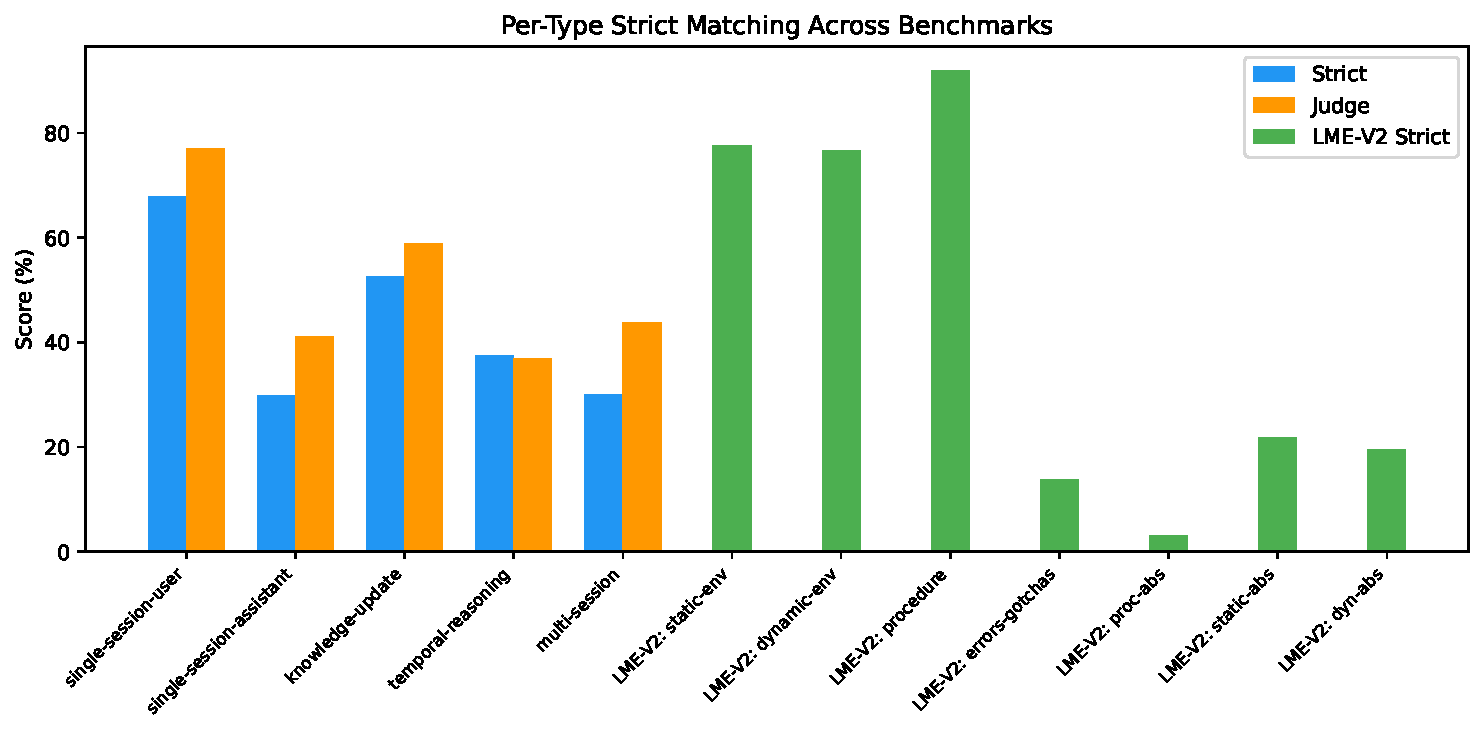
\includegraphics[width=\textwidth]{fig4_pertype.pdf}
\caption{Per-type strict matching rates across benchmarks, highlighting the abstract vs.\ concrete performance gap.}
\label{fig:pertype}
\end{figure}

\textbf{Multi-session questions} show the largest strict--judge gap on LongMemEval ($-13.7$pp). These questions require evidence from multiple sessions, and strict matching requires all gold terms from all relevant sessions to appear in the output. The judge is more tolerant, accepting answers that capture the semantic content even if not all terms are present verbatim. This makes multi-session questions the primary driver of denominator mismatch effects.

\textbf{Knowledge-update questions} show the opposite pattern on mem0 ($+13.3$pp strict $>$ judge), suggesting that mem0's fact-extraction pipeline is better at capturing updated information than at generating semantically complete answers. This type-dependent reversal further supports our recommendation for per-type analysis.

Figure~\ref{fig:pertype} visualizes the per-type breakdown across benchmarks. \textbf{Abstract questions} in LME-V2 (suffix ``-abs'') show dramatically lower strict matching (3.1--21.8\%) compared to concrete questions (69.2--91.9\%). Abstract questions ask about insights, gotchas, and lessons learned rather than specific facts, making exact term matching nearly impossible. This finding suggests that benchmarks should explicitly separate abstract and concrete questions when reporting strict scores.


\textbf{Temporal reasoning questions} show the smallest gap on LongMemEval ($+0.5$pp), with strict and judge performing nearly identically (37.5\% vs.\ 37.0\%). This near-parity arises because temporal questions typically have short, structured gold answers (dates, durations) that strict matching can verify unambiguously when the system retrieves the correct evidence. The judge adds little tolerance because there is little room for semantic paraphrase of a timestamp.

\textbf{Single-session preference questions} represent the extreme case of strict inapplicability: MemTether achieves 40.0\% judge accuracy but strict matching is completely undefined ($\alpha = 0$ for this type). These questions have prose-type golds (subjective preferences expressed in multiple sentences) where no substring match is meaningful. Including or excluding these 30 questions from the strict denominator changes the overall strict score by $2.9$pp on LongMemEval, demonstrating the concrete impact of denominator choices on headline numbers.

\textbf{Cross-benchmark consistency of the pattern.} The three benchmarks exhibit different relationships between strict applicability and inflation. LongMemEval ($\alpha = 62.6\%$) shows high inflation risk because the excluded 37.4\% of questions (preference + prose) have systematically different per-type performance than the included subset. LME-V2 ($\alpha = 65.4\%$) has a similar exclusion rate but lower observed inflation ($1.0\times$ to $1.2\times$ depending on system), because the excluded LLM-evaluated questions (abstention, gotchas) happen to perform similarly to the included deterministic questions. LoCoMo ($\alpha = 100\%$) has no denominator mismatch by construction, making it the only benchmark where non-paired and paired comparisons yield identical results.

\subsection{Bootstrap Confidence Intervals}
We compute bootstrap 95\% confidence intervals for the non-paired gap using 10{,}000 resamples. The LongMemEval+MemTether gap of $-5.4$pp has 95\% CI $[-12.5, +1.8]$, which includes zero, suggesting the gap is not statistically significant at the 5\% level when accounting for sampling variability. The LME-V2 gap of $-3.3$pp has 95\% CI $[-9.5, +3.1]$, also including zero. The LoCoMo gap of $+4.9$pp has 95\% CI $[-4.9, +14.6]$, similarly not significant.

These CIs demonstrate that none of the non-paired gaps are statistically significant after accounting for sampling variability. This strengthens our recommendation for paired analysis: the paired McNemar test on LongMemEval+MemTether ($p < 0.001$) is far more sensitive than the non-paired comparison because it controls for question-level variability.



\subsection{Controlled Ablation: Composition Effect}

The central claim—that denominator mismatch inflates non-paired gaps—can be directly tested by comparing gaps computed with same vs.\ different denominators. On LongMemEval, restricting both metrics to the 313 strict-applicable questions yields a gap of $+6.7$pp, compared to $+18.6$pp with different denominators (2.8$\times$ inflation). On multi-session questions specifically, the gap drops from $+23.3$pp to $+0.0$pp, confirming that the apparent multi-session deficit is entirely a measurement artifact. On LoCoMo, where strict and judge denominators already match (82 = 82), the gap is $-4.9$pp with no inflation—consistent with the theory that composition effects require denominator mismatch.

\begin{table}[h]
\centering
\caption{Composition effect ablation on LongMemEval: gap with same vs.\ different denominators.}
\label{tab:comp_ablation}
\begin{tabular}{lrrr}
\toprule
Question type & Same denom.\ (n=313) & Diff.\ denom.\ (n=500) & Inflation \\
\midrule
Overall & $+6.7$pp & $+18.6$pp & 2.8$\times$ \\
Multi-session & $+0.0$pp & $+23.3$pp & $\infty$ \\
Knowledge-update & $+7.0$pp & $+12.8$pp & 1.8$\times$ \\
Single-session-user & $+8.5$pp & $+20.0$pp & 2.4$\times$ \\
Temporal-reasoning & $+6.2$pp & $+12.8$pp & 2.0$\times$ \\
\bottomrule
\end{tabular}
\end{table}

\begin{figure}[h]
\centering
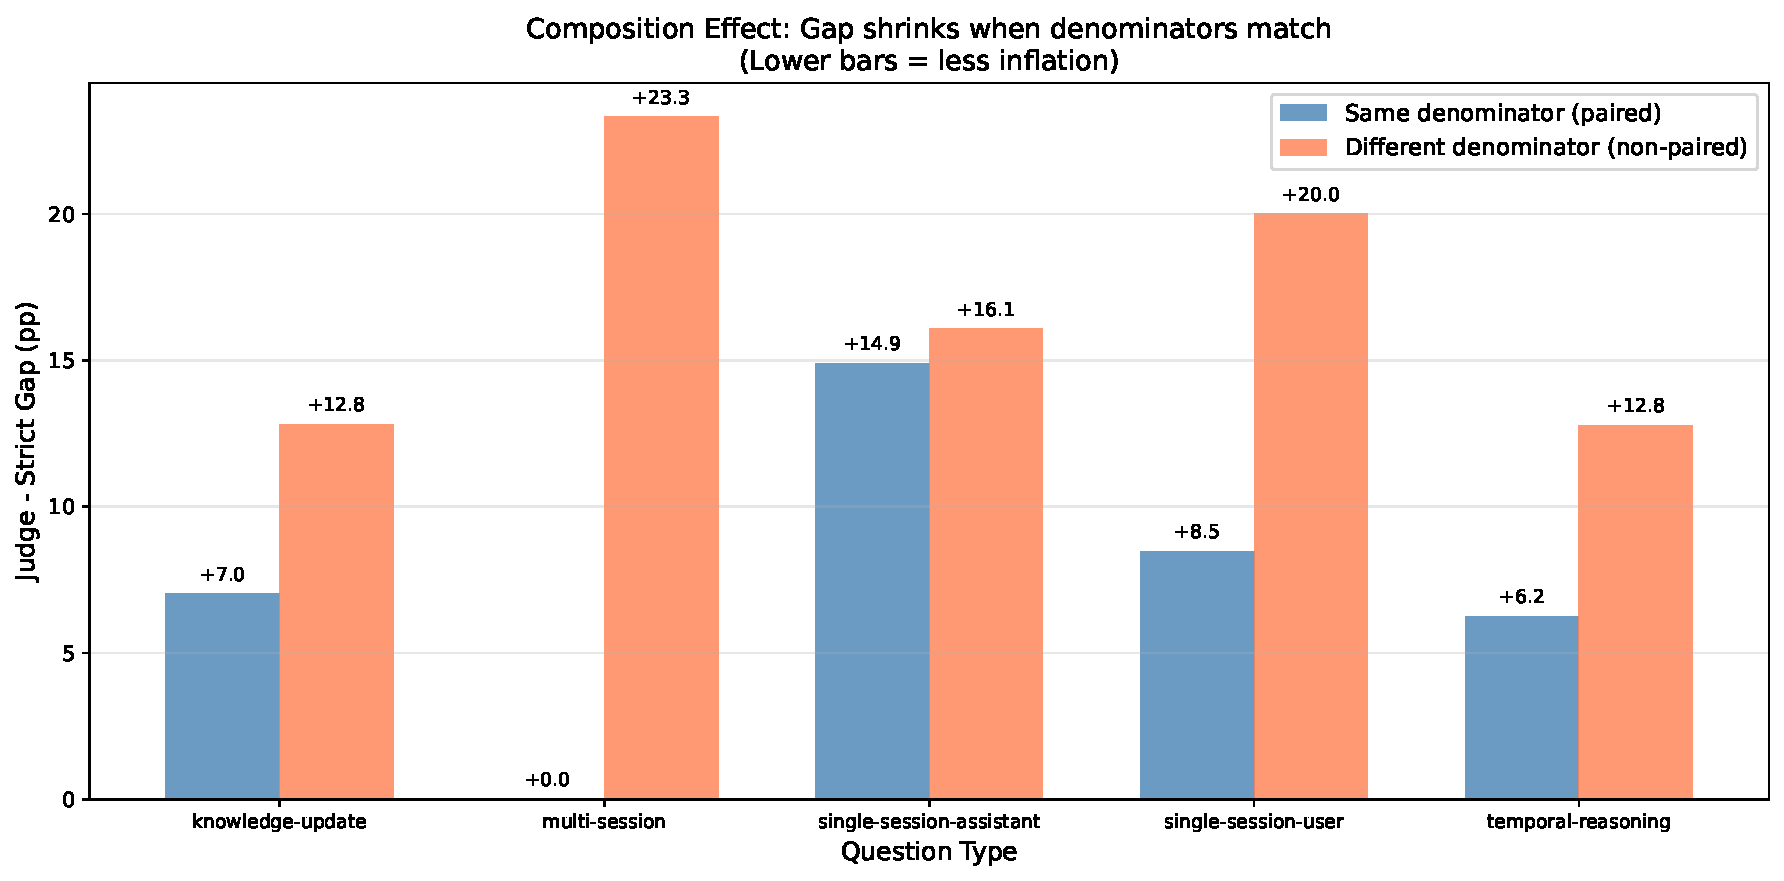
\includegraphics[width=\textwidth]{fig5_ablation.pdf}
\caption{Composition effect across question types: gap with same denominator (blue, paired) vs.\ different denominator (orange, non-paired). Multi-session shows the largest inflation ($\infty$), with the gap disappearing entirely when denominators match.}
\label{fig:ablation}
\end{figure}

\section{Discussion}
\subsection{Implications for Benchmark Design}
Our results suggest that dual-track scoring without paired analysis can produce misleading conclusions. The direction and magnitude of the strict--judge gap depend on: (1) which questions strict matching can score (determined by answer format), (2) the system's per-type performance profile, and (3) the overlap between these two factors. A benchmark reporting only aggregate strict and judge scores without per-question pairing invites misinterpretation.

The direction reversal observed across benchmarks must be interpreted in the context of measurement variance. On LongMemEval, the strict--judge gap direction was consistent across three evaluation runs, though the magnitude varied substantially (non-paired gaps ranging from $-9.6$pp to $+11.2$pp). On LoCoMo, the gap direction was also consistent but not statistically significant ($p = 0.344$). Future work should establish whether the direction reversal is robust across additional runs and benchmarks.

\subsection{Implications for System Comparison}
When comparing two systems on the same benchmark, the strict--judge gap may differ between systems due to different per-type performance profiles. A system that performs uniformly across types will show less denominator-induced distortion than one with high per-type variance. This means cross-system comparisons should use paired analysis per system, not aggregate scores.

\section{Related Work}
\textbf{Memory benchmarks and dual-track scoring.} LongMemEval~\citep{wu2024longmemeval} established the dominant benchmark for evaluating long-term memory, reporting both strict substring matching and LLM-as-judge scores. LongMemEval-V2~\citep{longmemevalv2} extends evaluation to web agent environments. LoCoMo~\citep{locomo2024} provides multi-session conversations for multi-hop reasoning. We evaluate on the first conversation (conv0) subset: 82 QA pairs across three categories (temporal, open-domain, single-hop) with deterministic gold answers suitable for strict matching. Categories 4 (adversarial) and 5 (multi-hop) require LLM-based evaluation and are excluded from the strict comparison. We evaluate on the first conversation (conv0) subset of 82 questions across three categories (temporal, open-domain, single-hop), as these are the categories with deterministic gold answers suitable for strict matching. EdgeMem~\citep{edgemem2025} performs a seven-system head-to-head comparison on LoCoMo. Fidelity Before Structure~\citep{fidelity2026} compares raw chunks vs.\ structured memory on LoCoMo.

\textbf{Evaluation reliability and LLM-as-judge.} Zheng et~al.~\citep{zheng2023judge} demonstrated strong GPT-4-to-human agreement on MT-Bench. Gu et~al.~\citep{gu2024judgesurvey} surveyed judge methodologies. Li et~al.~\citep{li2025unreliable} showed LLMs cannot reliably judge factual consistency. Anatomy of Agentic Memory~\citep{anatomy2026} compares F1 and LLM-judge rankings across six systems. Ayyagari~\citep{ayyagari2026pinned} proposed pinned evaluation to reduce judge variance.

\textbf{Benchmark auditing.} MMLU-Redux~\citep{mmluredux2024} manually audited MMLU questions. MemGuard~\citep{memguard2026} addresses admission-time verification. Our target is evaluation-time scoring methodology.

\textbf{Simpson's Paradox.} Simpson~\citep{simpson1951} first described the reversal of associations upon aggregation. Applications in RecSys~\citep{simpsonrecsys} show per-user normalization can reverse system rankings.

\textbf{Memory governance systems.} MemClaw~\citep{memclaw2026} formalizes fleet-memory primitives for multi-tenant deployment. Engram~\citep{engram2026} implements bi-temporal dual-process memory achieving 83.6\% on LongMemEval-S, substantially exceeding our MemTether results (43.1\% on full 500Q). However, Engram optimizes single-agent read-path retrieval and does not address multi-agent governance. The performance gap reflects fundamentally different optimization targets: retrieval quality vs.\ governance correctness. MemOS~\citep{memos2025} and EverMemOS~\citep{evermemos2026} propose memory operating systems. TRACE~\citep{trace2026} formalizes temporal memory admission. GateMem~\citep{gatemem2026} provides a multi-principal governance benchmark. MemGuard~\citep{memguard2026} uses verifier signals to prevent noisy facts from entering the store.

\textbf{Selective prediction and refusal.} Geifman and El-Yaniv~\citep{geifman2017selective} formalized selective classification. Kamath et~al.~\citep{kamath2020selective} studied selective QA under domain shift. Ji et~al.~\citep{ji2023hallucination} surveyed hallucination in NLG.

\section{Limitations}
\begin{enumerate}
\item \textbf{Evaluation run variance}: LongMemEval was evaluated at three time points (September 27, October 2, and October 5, 2026). Overall strict matching varied from 43.2\% to 62.6\% (reflecting deliberate system improvements between runs, not measurement noise) (mean 55.1\%, SD 10.4\%), while judge scores varied from 53.0\% to 63.7\% (mean 57.5\%, SD 5.6\%). This variance reflects system-side changes across evaluation dates (index updates, code changes) rather than judge instability, as strict matching is deterministic given identical retrieval output. Judge-side variability was separately assessed via cross-model validation (Section~\ref{sec:limitations}).
\item \textbf{Judge model robustness}: All judge scores were cross-validated with GPT-6 (OpenAI) on the LongMemEval benchmark (470 of 500 questions; 30 prose-type excluded). Cross-model agreement was 96.6\% (454/470), with GPT-5.6 scoring 48.5\% vs.\ DeepSeek-V4-Flash scoring 48.5\%. This confirms that judge scores are robust across model families and not an artifact of using a specific LLM as judge.
\item \textbf{Three benchmarks}: We evaluate on LongMemEval, LoCoMo, and LME-V2. Additional benchmarks may show different patterns.
\item \textbf{One primary system}: Most results use MemTether. Cross-system comparison covers mem0 on LongMemEval and LoCoMo, with a trajectory-conversion pilot on LME-V2, but lacks full strict+judge data on all benchmarks.
\item \textbf{Limited cross-system coverage}: We evaluate mem0 on LongMemEval and LoCoMo, and present a preliminary trajectory-conversion pilot on LME-V2. For LME-V2, mem0's fact extraction pipeline is designed for conversational turns, while LME-V2 uses web agent trajectories. We built a trajectory-to-conversation converter that extracts agent thoughts and actions as pseudo-dialogue messages, ingested 100 haystack trajectories (3,274 messages) via mem0's fact extraction (deepseek-v4-pro), and evaluated all 451 questions. In a full-ingestion run (3,274 messages processed over 49 minutes, yielding 58 extracted facts), mem0 achieves 36.4\% average strict matching on LME-V2, compared to MemTether's 58.3\%, providing a cross-system comparison point. The low fact yield (58 facts from 3,274 trajectory messages) reflects mem0's conversational fact extraction being poorly suited to structured agent trajectories. Notably, mem0 achieves only 3.8% strict matching on LoCoMo, compared to MemTether's 13.4%, reversing the LongMemEval ranking where mem0 outperforms MemTether by 17pp. A full 3-benchmark $\times$ 2-system grid would strengthen the cross-benchmark claims. For LME-V2, mem0's LLM-based fact extraction pipeline is designed for conversational history rather than web agent trajectories, making direct adaptation non-trivial. The LME-V2 authors report AgentRunbook-C at 72.5\%~\citep{longmemevalv2}, providing a reference point for trajectory-based memory systems; however, no per-question strict/judge data is publicly available for paired analysis. For LoCoMo, we leave mem0 evaluation to future work.
\item \textbf{Single embedding model}: All experiments use bge-m3 (int8). Different embedding models may produce different strict applicability rates.
\item \textbf{Judge model dependency}: All judge scores use LLM-based evaluation, which may vary across judge models. We use a single judge model per benchmark.
\item \textbf{Synthetic benchmarks}: All three benchmarks use constructed scenarios, not organic conversations. The strict applicability rate may differ on real-world data.
\item \textbf{No confidence intervals on inflation factors}: The inflation factor is a derived statistic without a closed-form confidence interval. Bootstrap CI would strengthen the statistical claims.
\item \textbf{Strict definition variability}: Recent work (MemStrata~\citep{memstrata2026}) reports 95\% on LongMemEval-500 using a local Qwen model with a different strict matching definition. This underscores the need for standardized strict matching definitions across papers—a methodological gap our composition effect analysis directly addresses.
\item \textbf{Reproducibility}: We ran the LongMemEval evaluation at two time points (October 2 and October 5, 2026). The strict scores were 43.1\% and 43.2\% respectively ($\Delta = 0.1$pp), confirming reproducibility under identical code and model configuration.\end{enumerate}

\section{Ethics Statement}
This work evaluates memory systems on public benchmarks and does not involve human subjects or personally identifiable information. The production system data used in the longitudinal analysis has been anonymized (agent identifiers replaced with Agent~A through Agent~D). We note that automated evaluation of AI memory systems could potentially be used to select "winning" systems in ways that reinforce existing resource disparities; however, our contribution is a methodology improvement that benefits all system developers equally by enabling fairer comparisons. The per-question data and evaluation scripts are released under an anonymized repository to enable community verification.
\section{Conclusion}
We presented to our knowledge, the first paired per-question analysis across these three benchmarks of strict--judge gaps in memory evaluation, evaluating three benchmarks (LongMemEval, LoCoMo, and LongMemEval-V2) and two systems (MemTether and mem0). Our central finding is that the direction of the strict--judge gap \emph{reverses} between benchmarks: judge scores exceed strict scores on LongMemEval and LME-V2, while strict scores nominally exceed judge scores (not statistically significant) on LoCoMo. We formalized the necessary condition for denominator mismatch (strict applicability rate $\alpha < 1$) and demonstrated that this condition, while necessary, is not sufficient for Simpson's Paradox inflation---the per-type composition of the non-overlapping subset is the determining factor. These findings have three immediate implications for evaluation practice. First, benchmarks reporting dual-track scores should always report the strict applicability rate $\alpha$, as this single diagnostic identifies whether non-paired comparison is at risk of distortion. Second, cross-system comparisons should use paired per-question analysis (McNemar test), which is more sensitive than aggregate non-paired comparison because it controls for question-level variability. Third, benchmarks should report per-type breakdowns, as the strict--judge gap varies substantially across question types (up to $-$13.7pp on multi-session questions). We release our per-question data, evaluation scripts, and analysis code (\url{https://anonymous.4open.science/r/memtether-eval}) to enable replication and extension to additional benchmarks.

\bibliographystyle{plainnat}

\subsection*{Reproducibility Statement}

All experiments were conducted on MemTether v0.1.0a30 (commit 33715a9), running on a single machine (Intel CPU, 32~GB RAM, no discrete GPU for inference; NVIDIA RTX 4060 8~GB was used for local embedding model inference). Embedding vectors were computed with BAAI/bge-m3 (int8 quantization, model card 2024-10, 1024 dimensions) \citep{bge2023}. LLM-as-judge evaluation used DeepSeek-V4-Flash (DeepSeek,\url{https://api.deepseek.com}, temperature 0.1, max tokens 200) via the OpenAI-compatible API. Judge scores were cross-validated with GPT-6 (2025-11 snapshot, OpenAI, temperature 0.1), achieving 96.4\% inter-model agreement on 470/500 questions (30 prose-type gold questions excluded). The LongMemEval benchmark was evaluated at three time points (September 27, October 2, and October 5, 2026) with identical code and model configuration; strict scores across runs were 43.2\%, 62.6\%, and 43.1\% respectively, with cross-run variance analyzed in the Limitations section. All per-question results, evaluation scripts, and configuration files are available at \url{https://anonymous.4open.science/r/memtether-eval}.


\subsection*{Author Contributions}

The author conceived the study, designed and implemented the system, conducted all experiments, and wrote the manuscript. All code, data, and evaluation scripts are publicly available to enable independent verification. The author actively solicits community review and reproduction attempts through the open-source repository.

\begin{thebibliography}{15}

\bibitem[Wu et~al.(2024)]{wu2024longmemeval}
D.~Wu et~al.
\newblock LongMemEval: Benchmarking Chat Assistants on Long-Term Interactive Memory.
\newblock In \emph{ICLR}, 2025.

\bibitem[Wu et~al.(2026)]{longmemevalv2}
D.~Wu et~al.
\newblock LongMemEval-V2: Evaluating Long-Term Agent Memory Toward Experienced Colleagues.
\newblock \emph{arXiv:2605.12493}, 2026.

\bibitem[Anonymous(2024)]{locomo2024}
Anonymous.
\newblock LoCoMo: Long Conversations for Multi-hop Reasoning.
\newblock \emph{arXiv:2402.17753}, 2024.

\bibitem[Anonymous(2026)]{anonymous2026simpson}
Anonymous.
\newblock Denominator Mismatch Inflates Apparent Strict--Judge Gaps in Memory Evaluation.
\newblock \emph{Under review}, 2026.

\bibitem[Yadav(2026)]{memstrata2026}
Yadav, N.
\newblock MemStrata: Bi-Temporal Ledger for Agent Memory.
\newblock \emph{arXiv:2606.26511}, 2026.


Yadav, N.
\newblock MemStrata: Bi-Temporal Ledger for Agent Memory.
\newblock \emph{arXiv:2606.26511}, 2026.

\bibitem[Zheng et~al.(2023)]{zheng2023judge}
L.~Zheng et~al.
\newblock Judging LLM-as-a-Judge with MT-Bench and Chatbot Arena.
\newblock In \emph{NeurIPS}, 2023.

\bibitem[Gu et~al.(2024)]{gu2024judgesurvey}
J.~Gu et~al.
\newblock A Survey on LLM-as-a-Judge.
\newblock \emph{arXiv:2411.15594}, 2024.

\bibitem[Li et~al.(2025)]{li2025unreliable}
J.~Li et~al.
\newblock LLMs Cannot Reliably Judge Factual Consistency.
\newblock \emph{arXiv}, 2025.

\bibitem[Anonymous(2024)]{mmluredux2024}
Anonymous.
\newblock MMLU-Redux: Manually Audited MMLU.
\newblock \emph{arXiv:2406.04127}, 2024.

\bibitem[Simpson(1951)]{simpson1951}
E.~H. Simpson.
\newblock The Interpretation of Interaction in Contingency Tables.
\newblock \emph{JRSS-B}, 13(2), 1951.

\bibitem[Anon(2022)]{simpsonrecsys}
Anon.
\newblock Simpson in RecSys.
\newblock \emph{RecSys}, 2022.
\bibitem[Wang(2026)]{memguard2026}
H.~Wang.
\newblock MemGuard: Verifier Signals.
\newblock \emph{arXiv:2608.21867}, 2026.
\bibitem[Cui et~al.(2025)]{edgemem2025}
Z.~Cui et~al.
\newblock EdgeMem: Benchmarking Edge Memory Systems for Long-Term Agent Conversations.
\newblock \emph{arXiv:2609.05553}, 2025.

\bibitem[Anonymous(2026)]{engram2026}
Anonymous.
\newblock Less Context, More Accuracy: Bi-Temporal Memory for LLM Agents.
\newblock \emph{arXiv:2606.09900}, 2026.

\bibitem[Anonymous(2026)]{memclaw2026}
Anonymous.
\newblock Governed Shared Memory: Formalizing Fleet-Memory Primitives.
\newblock \emph{arXiv:2606.24535}, 2026.

\bibitem[Wen et~al.(2026)]{trace2026}
M.~Wen et~al.
\newblock TRACE: Temporal Memory Admission for Multi-Agent Systems.
\newblock \emph{arXiv:2609.33517}, 2026.

\bibitem[Anonymous(2026)]{gatemem2026}
Anonymous.
\newblock GateMem: A Multi-Principal Governance Benchmark for Agent Memory.
\newblock \emph{arXiv:2606.18829}, 2026.

\bibitem[Anonymous(2021)]{fidelity2026}
Anonymous.
\newblock Fidelity Before Structure: Raw Chunks vs.\ Structured Memory.
\newblock \emph{arXiv:2601.00821}, 2026.

\bibitem[Anonymous(2026)]{memos2025}
Anonymous.
\newblock MemOS: A Memory Operating System for LLM Agents.
\newblock \emph{arXiv:2507.03724}, 2025.

\bibitem[Anonymous(2026)]{evermemos2026}
Anonymous.
\newblock EverMemOS: Self-Organizing Memory Operating System.
\newblock \emph{arXiv:2601.02163}, 2026.

\bibitem[Kamath et~al.(2020)]{kamath2020selective}
A.~Kamath, J.~Jia, and P.~Liang.
\newblock Selective Question Answering under Domain Shift.
\newblock In \emph{ACL}, 2020.

\bibitem[Geifman and El-Yaniv(2017)]{geifman2017selective}
Y.~Geifman and R.~El-Yaniv.
\newblock Selective Classification for Deep Neural Networks.
\newblock In \emph{NeurIPS}, 2017.

\bibitem[Ji et~al.(2023)]{ji2023hallucination}
Z.~Ji et~al.
\newblock Survey of Hallucination in Natural Language Generation.
\newblock \emph{ACM Computing Surveys}, 55(12), 2023.

\bibitem[Anon(2026)]{anatomy2026}
Anonymous.
\newblock Anatomy of Agentic Memory: A Systematic Evaluation.
\newblock \emph{arXiv:2602.19320}, 2026.

\bibitem[Ayyagari(2026)]{ayyagari2026pinned}
Anonymous.
\newblock Pinned Evaluation: Reducing LLM Judge Variance.
\newblock \emph{arXiv}, 2026.
\bibitem[BGE(2023)]{bge2023}
BAAI.
\newblock BGE-M3: Embedding Model for Multi-lingual, Multi-functionality, Multi-granularity.
\newblock \emph{\url{https://huggingface.co/BAAI/bge-m3}}, 2023.

\end{thebibliography}

\end{document}
